\documentclass{article}

\usepackage[margin=1in]{geometry}
\usepackage{graphicx}
\usepackage{hyperref}
\usepackage{pgfgantt}

\title{The Gentrification of the San Francisco Bay Area \\ \large TEAM-17 Progress Report}
\author{Benicio Bailey, Jacob Feenstra, Diane Kim, Aryan Sarda}

\begin{document}
\maketitle

\section{Method}

 We will list out the primary components  of the visualization here (which is essentially complete). It is broken into 3 main components, with the third component housing most of the visualization. We'll discuss overall design, before getting into what has been implemented so far. Then, we'll touch on how it tells the story, as well as what has changed in the design since our proposal.

\subsection{Current Design}

\begin{description}

    \item[Introduction:] After feedback from Professor Liu, we have decided to begin with a martini glass-like introduction, while still retaining our fully exploratory \& interactive drill-down map. It will highlight the purpose of the visualization, and interaction tips, before releasing the user to freely explore the Bay Area gentrification map.
    
    \item[Bay Area Map:] In the 9-county view of the bay area (see Figure~\ref{fig:first}), the user will be able to select one of the 9 counties presented. This aspect of the visualization is pretty simplified, beyond making it clear that the counties can be selected.
    
    \item[County Heatmap:] Here is where the visualization gets complicated; it is portrayed in Figure~\ref{fig:second}. We walk through it's various features below.
    
    \begin{description}
    
        \item[Census Tract Heatmap:] Perhaps the most advanced part of the entire project, the census tracts of a county are represented on a heatmap. It's a conventional 2-color heatmap from white to red; white represents no gentrification in a given county tract, whereas red indicates extreme gentrification. Most census tracts will fall somewhere in-between. Grey census tracts indicate incomplete criteria. By hovering over a census tract, the user can see the various attributes for a given census tract: it's Median Home Value, Median Household Income, Occupancy Status (also known as Vacancy Status), Gross Rent, Population, and Educational Attainment.  
        
        \item[2010-2023 Timeline:] Just as important as the gentrification criteria themselves is visualizing how they \textit{change} over the years. The user interacts with a slider defined for 2010 to 2023, and the census tract's year corresponds to the year on the slider. The heatmap changes in "real-time", and the user is able to see how particular communities change in their gentrification criteria (with the heatmap).
        
        \item[Vis Dashboard:] A dashboard lies adjacent to the heatmap, as seen on the right-hand side of Figure~\ref{fig:second}. Using secondary visualizations to provide context for the heatmap, it consists of the following components.
        
        \begin{description}
        
            \item[Timeline Annotations:] One section of the dashboard consists of timeline annotations, providing context for what occurred in the given year to corroborate shifts in gentrification, and guiding the user to glean insights from the data. It will comprise a few salient bulletpoints. For interim/lull years, this will be indicated, if there are no significant events on the timeline. Figure~\ref{fig:second} shows "What Happened in Year?", but this formatting will likely change slightly in the final stages. These annotations will shift year-to-year to significant events that happened in the county. If they are particularly related to a specific part in the county map, there may be a point of interest system related to these annotations, but this is still being prototyped.
            
            \item[Stream Graph:] To quickly ascertain how the gentrification criteria changes over the years (the heatmap, while interactive \& intuitive, doesn't really encode \textit{how} the data changes in one viewing window), a stream graph will show how the 6 attributes change from 2010-2023 for a selected census tract. If the user clicks on a census tract, then the stream graph will chart the change in gentrification criteria for this given census tract. This is abstractly represented in the middle of the dashboard in Figure~\ref{fig:second}.
            
            \item[Comparative Bar-Chart:] For the six attributes of the dataset, we have a small bar-chart that shows the average of the six attributes (across all census tracts for selected county) for the given year. This gives the user a quick snapshot of whether or not these values are increasing or decreasing year-to-year. Heatmaps are large, and a user cannot always immediately ascertain if gentrification has increased from one year to the next. This simple bar chart will clue the user in on heatmap trends, but it is not intended to be viewed in isolation. 
            
        \end{description}
        
    \end{description}
    
\end{description}

\graphicspath{{../imgs/}}

\begin{figure}[h!]
    \centering
    \begin{minipage}{0.48\textwidth}
        \centering
        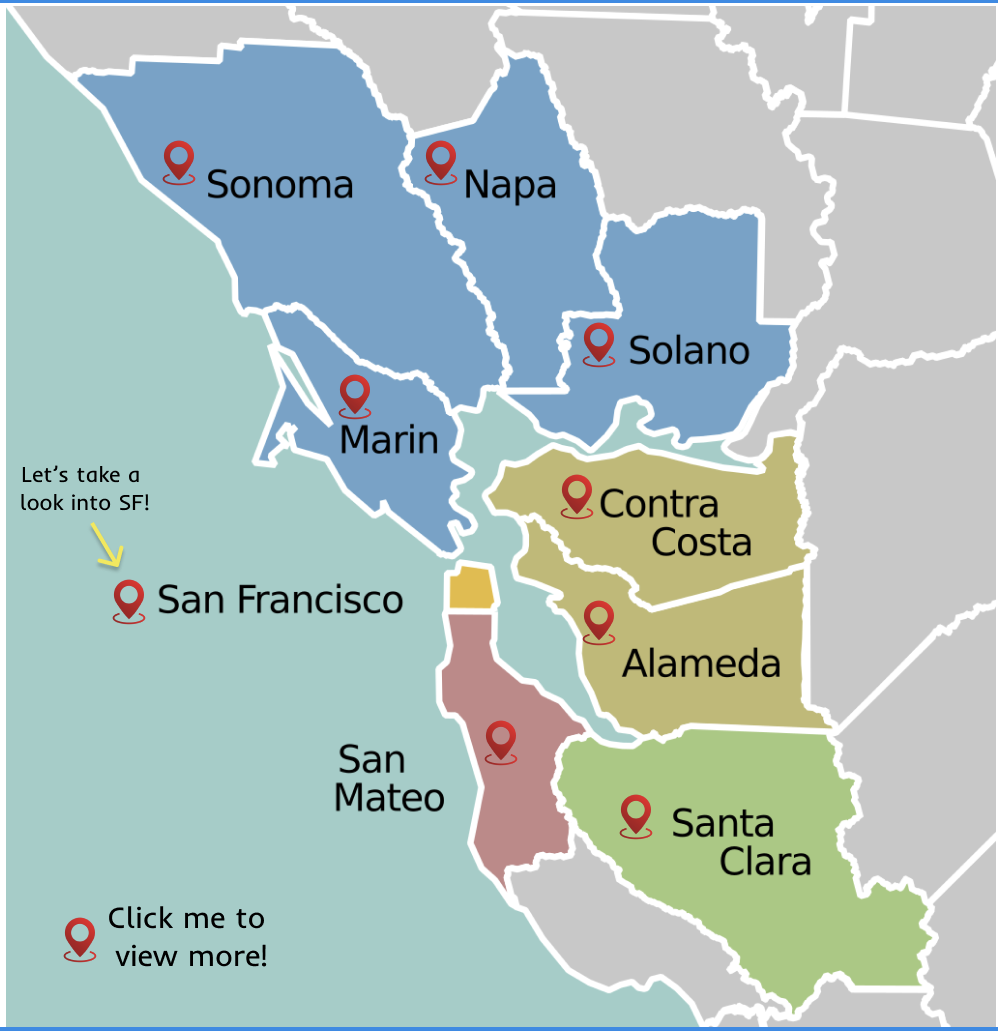
\includegraphics[width=\linewidth]{fig1.png}
        \caption{View of the Bay Area}
        \label{fig:first}
    \end{minipage}\hfill 
    \begin{minipage}{0.48\textwidth}
        \centering
        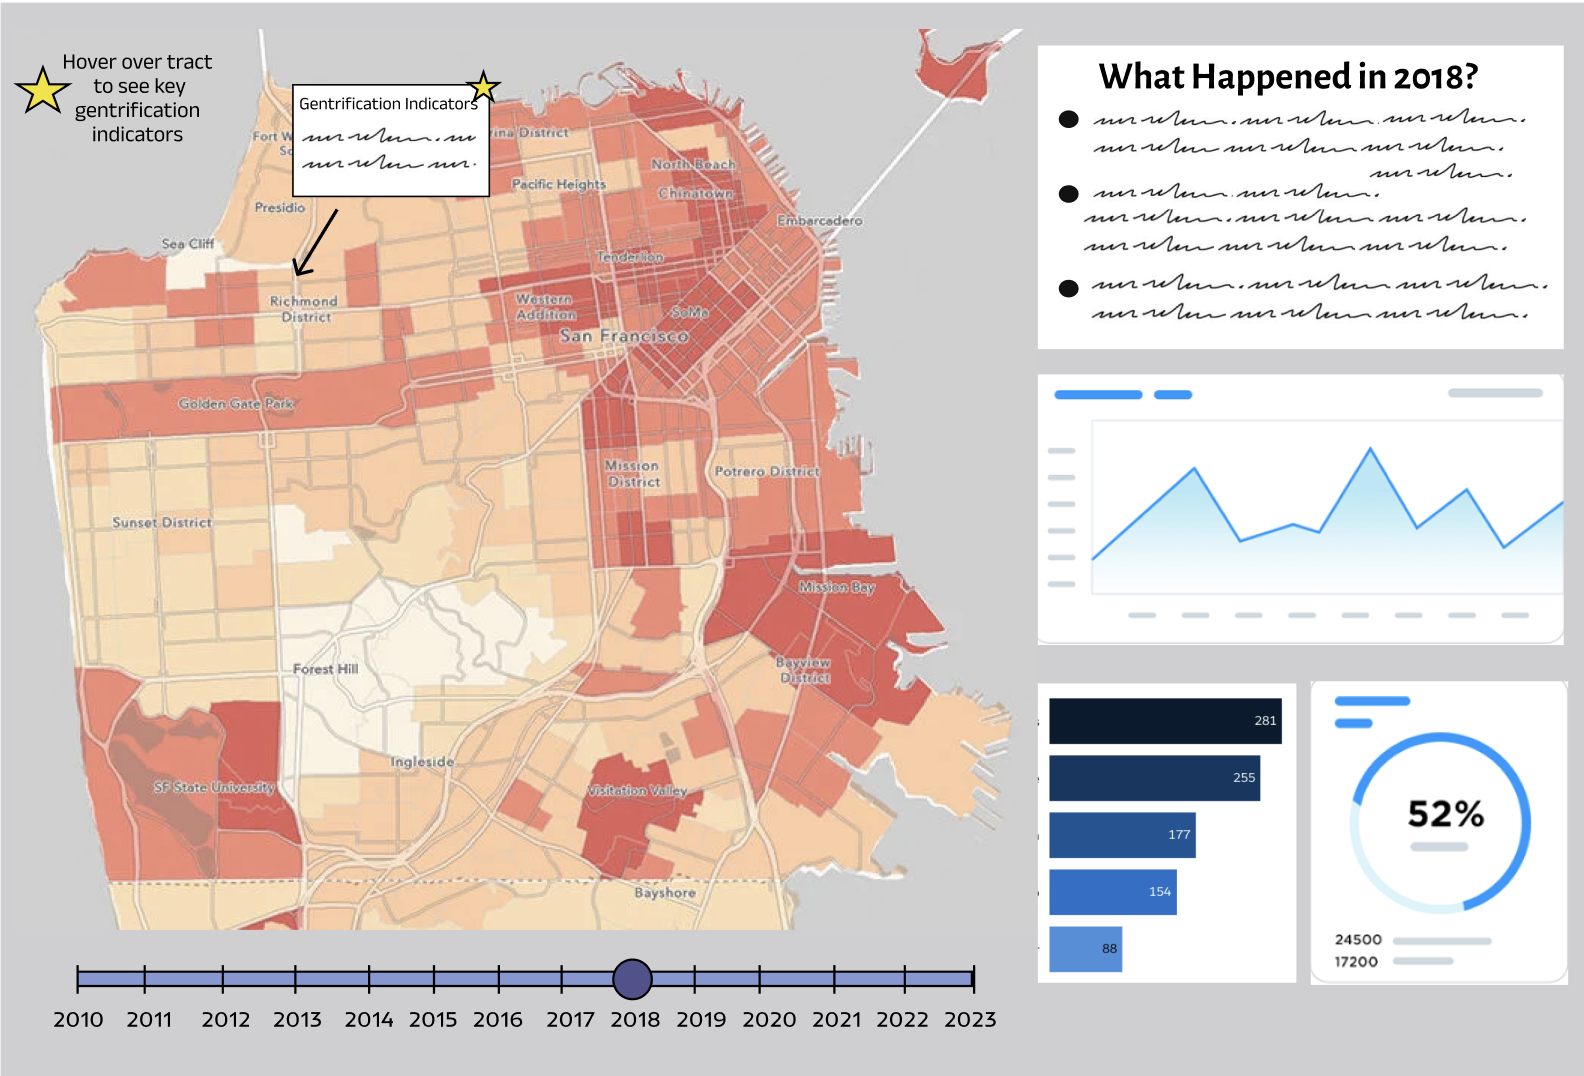
\includegraphics[width=\linewidth]{fig2.png}
        \caption{View of San Francisco County, by census tract}
        \label{fig:second}
    \end{minipage}
    \caption{Drill-Down approach to explore Bay Area counties}
    \label{fig:combined}
\end{figure}

\subsection{Implementation}

\begin{description}

    \item[Introduction:] The script for the martini-glass like introduction is written, but it still needs to be visualized in a separate D3 js visualization. It will consist of the script, images if they are needed, and a button to advance to the bay area map.
    
    \item[Bay Area Map:]  In order to get a map that correctly displays all our data to it's corresponding geographic location, we required a TopoJSON file that has information regarding each census tract. We have found a file for all states, counties, and tracts in the United States and preprocessed the data into a smaller file with TopoJSON data for the bay area counties we will focus on. Currently, there is a working map that identifies counties when hovering over them, but we still need to polish UI/UX, and include transitions into visualization for specific counties.
        
    \item[County Visualization:] \hfill
    
    \begin{description}
    
        \item[Census Tract Heatmap:] We have not started implementing the county heatmaps yet, but have prepared the county heatmap images which will have the heatmaps applied to them.
        
        \item[2010-2023 Timeline:] The timeline slider lets users select a year between 2010-2023, with the heatmap updating in real time based on the selected year’s data. Each year corresponds to a separate layer of our gentrification dataset, preprocessed and indexed for efficient switching. The slider will sit horizontally beneath the heat map and include a label  to show the active year. When the year changes, a function is designed to update the fill color of each census tract based on that year’s gentrification values. Once the heatmap is implemented, we plan to apply this color-changing logic to verify its behavior with the full dataset. To make these transitions smoother, we’ll apply D3's fade effects. We also plan to sync the slider with dashboard annotations for each year. So far, the timeline element has been added and is transitioning, but the heatmaps aren't in-place yet.
        
        \item[Vis Dashboard:] \hfill
        
        \begin{description}
        
            \item[Timeline Annotations:] Research still needs to be finished for timeline annotations. The visualization aspect for these are at a reduced level; implementation will mostly consist of refining the text and adding where appropriate for each year.
            
            \item[Stream Graph:] The stream graph has not been visualized yet, but all of the data is prepared, and visualization should be straight-forward after the heatmap is implemented.
            
            \item[Averages Bar Chart:] The bar chart has not been implemented, but the underlying dataset is prepared, and the visualization idiom should be trivial. 
            
        \end{description}
        
    \end{description}
    
\end{description}

\subsection{Storytelling Aspects}

The storytelling of the project is bolstered by three key pieces: the introduction, timeline annotations, and composite data. The introduction will clue the user in on how to navigate our visualization, and importantly for the storytelling aspect, the kind of insights and shifts in data to look out for! The timeline annotations will support the gentrification criteria as it changes year-to-year. It will be very important in telling the story on a more granular scale; these annotations will also expand the scope whenever possible, to tie it to our main story of gentrification in the SF Bay Area. In terms of the data itself, it will be important that we get the composite picture of the data just right. When the user looks at the heatmap, combined with the visualization dashboard, and the interactive tools we offer, it will be crucial that all of it be synthesized into a singular complete story. Each aspect of the data being visualized should support the other. We believe the heatmap-dashboard approach, combined with the timeline, will achieve this.
    
\subsection{Design Changes}

Since our proposal report, the 2 most significant changes are the introduction visualization and the county dashboard. The introduction will help solidify the purpose and intent of our visualization, and we have laid out what the county dashboard will analyze; namely the stream graph and the bar chart (as discussed earlier in the report).

\section{Evaluation Plan}

Team 17 intends to have a testing \& review session during the last couple of days before finalizing submission. First, each of the five team-members will walk through all aspects of the visualization in one sitting, noting inconsistencies or things that differ from the project's vision. This will be done independently for maximum coverage. Then, if we have time, we will address these inconsistencies. Secondly, we'll compare visualization against proposal report \& team member slideshow. Have we covered everything that we wanted to visualize? What are we missing? How? Have we fallen short in some aspects of the visualization? See how much fidelity our visualization has with respect to the original source material. We will pay attention to the relevant questions and theses asked, and whether the present visualization captures them. Finally, we'll refer to feedback received from T/A's and Professors as we continue to finalize project development; either from the reports, the slideshow, or during office hours.
    
\section{Preliminary Results}

We do not have conclusive reports/insights so far. The heatmap is not finished, and the timeline annotation research has not been fully conducted. Once we have completed both of these in the next week, all of our insights will be delineated in our final report. Note this is also why there is not an abundance of references in this report; we have amassed a large amount of sources and articles that cover bay area gentrification \& housing, but we need to narrow it down to only especially pertinent articles for timeline annotations (as well as the introduction). All sources for these annotations will be cited in the final report. 

\section{Plan of Activities}

The following Gantt chart illustrates the timeline of key project tasks, when they are occurring, who is primarily responsible for them, and their progress. Note that since this is a team project, everyone will likely contribute to every aspect of the project in some way. The singular names indicate who has been assigned to oversee an aspect of the project.

\begin{center}
\begin{ganttchart}[
  hgrid,
  vgrid,
  time slot format=isodate,
  time slot unit=day,
  x unit=0.7cm,
  y unit chart=0.8cm,
  title/.style={draw=none, fill=gray!20},
  title label font=\bfseries\footnotesize,
  bar/.style={fill=blue!50},
  bar label font=\small\color{black},
  bar label node/.append style={align=center, text width=4.5cm},
  bar height=0.6,
]{2025-05-21}{2025-06-05}

\gantttitle{Project Timeline}{16} \\
\gantttitlecalendar{month=name, day=2} \\

\ganttbar[
  progress=100
]{data preprocessing\\(Jacob)}{2025-05-21}{2025-05-23} \\

\ganttbar[
  progress=100
]{progress report\\(Jacob)}{2025-05-23}{2025-05-26} \\

\ganttbar[
  progress=0
]{video presentations\\(all)}{2025-06-02}{2025-06-05} \\

\ganttbar[
  progress=40
]{timeline annotations\\(Jacob)}{2025-05-26}{2025-06-02} \\

\ganttbar[
  progress=50
]{martini glass intro\\(Jacob)}{2025-05-26}{2025-06-01} \\

\ganttbar[
  progress=10
]{bay area map \& interactivity\\(Aryan)}{2025-05-23}{2025-06-02}\\

\ganttbar[
  progress=0
]{json county maps\\{(Benicio)}}{2025-05-23}{2025-05-28} \\

\ganttbar[
  progress=10
]{county vis dashboard\\(Diane)}{2025-05-23}{2025-06-03} \\

\ganttbar[
  progress=20
]{9 census tract heatmaps\\(Benicio)}{2025-05-23}{2025-06-03} \\

\ganttbar[
  progress=10
]{2010-2023 timeline\\(Diane)}{2025-05-23}{2025-06-03} \\

\ganttbar[
  progress=0
]{testing \& review\\(all)}{2025-06-03}{2025-06-04} \\

\ganttbar[
  progress=0
]{final report\\(Jacob)}{2025-06-01}{2025-06-05} \\

\end{ganttchart}
\end{center}

Note that this plan of activities is dynamic and will potentially change as the needs of our project change going into the final 10 days of development.

\section{Team's Effort Division}

Team 17 feels that every member of the team has contributed satisfactorily to our Bay Area Gentrification project, serving in different roles and capacities as the need arose.

\nocite{*}
\bibliographystyle{alpha}
\bibliography{refs}

\end{document}
